\documentclass[a4paper, 12pt, brazil]{article}

\usepackage[utf8]{inputenc}
\usepackage{amsmath,amssymb}
\usepackage{graphicx}
\usepackage{subfig}
\usepackage[colorinlistoftodos]{todonotes}
\usepackage{multirow}
\usepackage{indentfirst}
\usepackage{verbatim}
\usepackage{textcomp}
\usepackage{gensymb}
\usepackage{relsize}
\usepackage{setspace}
\usepackage[brazil]{babel}

\usepackage{lipsum}% http://ctan.org/pkg/lipsum
\usepackage{xcolor}% http://ctan.org/pkg/xcolor
\usepackage{xparse}% http://ctan.org/pkg/xparse
\NewDocumentCommand{\myrule}{O{1pt} O{2pt} O{black}}{%
  \par\nobreak % don't break a page here
  \kern\the\prevdepth % don't take into account the depth of the preceding line
  \kern#2 % space before the rule
  {\color{#3}\hrule height #1 width\hsize} % the rule
  \kern#2 % space after the rule
  \nointerlineskip % no additional space after the rule
}
\usepackage[section]{placeins}
\usepackage{booktabs}
\usepackage{colortbl}%
   \newcommand{\myrowcolour}{\rowcolor[gray]{0.925}}
   
\usepackage[obeyspaces]{url}
\usepackage{etoolbox}
\usepackage[colorlinks,citecolor=black,urlcolor=blue,bookmarks=false,hypertexnames=true]{hyperref} 

\usepackage{geometry}
\geometry{
	paper=a4paper, % Change to letterpaper for US letter
	inner=3cm, % Inner margin
	outer=3cm, % Outer margin
	bindingoffset=.5cm, % Binding offset
	top=2cm, % Top margin
	bottom=2cm, % Bottom margin
	%showframe, % Uncomment to show how the type block is set on the page
}

\begin{document}
\onehalfspacing
\begin{titlepage}
\begin{center}
\textbf{\large UNIVERSIDADE FEDERAL DE OURO PRETO}\\[0.3cm] 
\textbf{\large ESCOLA DE MINAS - Engenharia de Minas}\\[0.2cm]
\vspace{30pt}

\includegraphics{logoufop.jpg}\\[1cm]
\vspace{20pt}
\textbf{\large CAT124 - ELETROTÉCNICA GERAL}\\
\vspace{15pt}
\myrule[1pt][7pt]
\vspace{15pt}
\textbf{\large  DESENVOLVIMENTO DE UM MOINHO DE BOLAS PARA LABORATÓRIO}\\
\vspace{15pt}
\myrule[1pt][7pt]
\vspace{45pt}
\textbf{\large Alunos}\\[0.2cm]
Danilo de Almeida Silami \\[0.1cm]
Danilo de Vilhena Ayres Rodrigues \\[0.1cm]
Pedro Henrique Irene Bruno \\ 
\vspace{45pt}
\textbf {\large Professor:}\\[0.2cm]
\Large {Me. Danny A. T. Tonidandel}\\[0.1cm]
\end{center}
\end{titlepage}
\newpage
\section{Introdução}
A moagem é uma importante etapa no processo de beneficiamento mineral, pois além de estar relacionada com o gasto energético, uma área que requer grandes investimentos, é a etapa em que se define a granulometria que alimentará as etapas seguintes¹.
\newline

O moinho de bolas é uma máquina utilizada em processos de moagem. Trata-se de um dispositivo que, por meio de rotação, promove a sucessiva colisão de esferas, causando a cominuição de um determinado material².
\newline

Para um funcionamento adequado do equipamento faz-se necessário o uso de um motor que tenha potência necessária para rotacionar a carga formada pela estrutura do jarro de suporte, somada à sua carga interna. Um motor de um moinho de bolas deve ser preferencialmente de regime contínuo, o que significa que ele opera realizando trabalho durante muito tempo, mantendo sua temperatura sob equilíbrio².
\newline

Este projeto visa a fabricação de um moinho de bolas \ \textit{homemade}, de baixo custo, para cominuição de materiais em escala laboratorial, utilizando um motor de corrente alternada, monofásico, de regime contínuo, de baixa rotação

\section{Materiais e Métodos}
	\subsection{Materiais}
A Figura~\ref{fig:moinho} mostra a representação esquemática de um moinho de bolas descrito por de Paula et al. (2014)², que será utilizado de base para o desenvolvimento deste projeto.
	\begin{figure}[!ht]
 			\begin{center}
				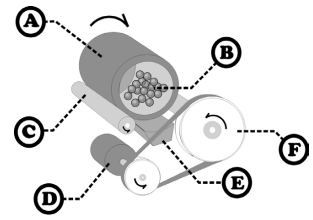
\includegraphics[width=100mm,scale=0.5]{moinho.png}
			\end{center}
       		\caption{\label{fig:moinho} Representação esquemática de um moinho de bolas. A) Jarro de moagem; B) Meio de moagem (esferas); C) Rolos; D) Motor; E) Correia; F) Polia (de Paula et al., 2014).}
 	\end{figure}
    
Para a confecção do Jarro (A) será utilizado um tubo de PVC cilíndrico com dimensões definidas ao longo do desenvolvimento. Serão utilizadas bolas de diferentes dimensões, estabelecidas ao longo do desenvolvimento do projeto. Serão utilizados dois eixos para o movimento do moinho e um sistema de correia-polias associado a um motor com características definidas ao longo do projeto.
\subsection{Metodologia} 
Silva (2014)¹ pontua os principais parâmetros observados na fabricação do moinho:
     \begin{itemize}
     	\item L/D (Razão entre as dimensões): é função do grau de finura desejada para o produto moído, e pode variar entre 1 e 5;v
        \item Em plantas de processamento os moinhos usados são do tipo overflow que operam a úmido e tem L/D entre 1 e 2,5
        \item Trabalha em velocidades de rotação maiores que as usadas nos moinhos de barras;
        \item Máquina para circuito fechado
     \end{itemize}
\par
A partir da determinação das dimensões de cada componente em conformidade com os materiais disponíveis no mercado, será determinada a velocidade de rotação do moinho. A velocidade de rotação tem relação direta com as dimensões do moinho e as características da carga interna do sistema. A equação~\ref{eq1} mostra a equação utilizada para a determinação da velocidade crítica (Vc) dada em rpm.

\begin{equation}
V_c=\frac{60}{2\pi}\sqrt{\frac{g}{R-r}}
\label{eq1}
\end{equation}

onde g é a gravidade (cm/s2), R é o raio do moinho (cm), e r o raio das esferas de moagem (cm). Recomenda-se trabalhar-se com velocidades cerca de 60 a 70\% da velocidade crítica, uma velocidade razoável de trabalho seria entre 68 e 80 rpm.
\newline

A escolha do motor, nesta aplicação, será de acordo com de Paula et al., (2014), utilizando um motor de corrente alternada, monofásico, de regime contínuo, de baixa rotação, mostra-se uma escolha bastante adequada. Motores de corrente alternada estão disponíveis para potências maiores, a custos mais acessíveis.
\newline

Para definir a potência do motor é necessário determinar o torque exigido pela carga, ou a curva de carga do equipamento. Uma estimativa segura para calcular o torque necessário é admitindo a situação na qual toda a carga do moinho encontrasse na extremidade lateral, exemplificada na Figura~\ref{fig:potencia}, e a equação~\ref{eq2} mostra o cálculo utilizado para obtenção da potência necessária ao sistema.

\begin{figure}[!ht]
 			\begin{center}
				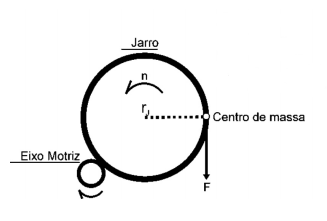
\includegraphics[width=100mm,scale=0.5]{potencia.png}
			\end{center}
       		\caption{\label{fig:potencia}Esquema do cálculo da potência útil do motor utilizado.}
 	\end{figure}   

\begin{equation}
P_u=(m.g)(r_j)(n.\frac{2\pi}{60})
\label{eq2}
\end{equation}

\par
onde P é a potência útil em W, m é a massa, em Kg, do sistema (jarro, esferas e amostra), g é a gravidade (m/s-2), rj o diâmetro do jarro (m), e n a rotação do jarro, em rpm.
\newline

Um sistema de redução de velocidade que funciona a partir de um sistema de polias que são responsáveis pelo ajuste de velocidade de trabalho do moinho. O dimensionamento adequado da redução das velocidades foi realizado pela relação velocidade angular/diâmetro: 

\begin{equation}
D_1.n_1=D_2.n_2
\end{equation}

\par
Será fabricada uma base estrutural de material definido ao longo do desenvolvimento onde serão acoplados os componentes do sistema (exceto o jarro). 

\newpage
\section{CRONOGRAMA}

\par
A tabela ~\ref{tab:Tabela 1} mostra o cronograma das atividades realizadas neste projeto.

\begin{table}[!ht]
        \caption{\label{tab:Tabela 1} \textbf{Cronograma de atividades}}
        \centering
\begin{tabular}{|c|c|c|c|c|}
\hline
\multirow{2}{*}{Ações} & \multicolumn{4}{c|}{Período (meses)} \\ \cline{2-5}
 & 1 & 2 & 3 & 4 \\ \hline
	Determinação das características dos componentes & \cellcolor[gray]{0.6} & &  & \\ \hline
	Aquisição dos materiais & & \cellcolor[gray]{0.6} & & \\ \hline
	Montagem do moinho & & \cellcolor[gray]{0.6} & \cellcolor[gray]{0.6} & \\ \hline
	Testes de funcionamento & & & & \cellcolor[gray]{0.6} \\ \hline
\end{tabular}
\end{table}

\newpage
\begin{thebibliography}{99}
    \bibitem{LPF}
    SILVA, J.A.O. \textbf{Modelagem do moinho de bolas de rocha fosfática da empresa anglo american fosfatos brasil utilizando a ferramenta moly-cop tools.} Monografia de especialização em tratamento de minérios. Universidade Federal de Goiás. Catalão, 2014. 
	\bibitem{HPF} 
	de PAULA, L.F.; ALVES, A.C.; ALVES, C.S.; RIBEIRO, E.A.; MADURRO, A.G.B.; MADURRO, J.M. \textbf{Diretrizes para a construção de um moinho de bolas para a moagem de sólidos em laboratórios.} Quim. Nova, Vol. 37, No. 4, 736-739, 2014.
\end{thebibliography}
\noindent
\end{document}